\section{Descriptive statistics of vulnerable resources}
\subsection{Country overview}
\autoref{fig:heatmap} presents geographic distribution of vulnerable resources. In highlighted countries, we detected at least one vulnerable server while the size of each circle is proportional to their number. We discovered vulnerable servers in 125 countries across the globe including all the countries in Europe, North America and a vast majority of countries in Asia, South America, Australia and Oceania. Relatively low number of vulnerable servers in the African region can be explained by low number of total DNS servers in the area \footnote{\url{https://labs.ripe.net/Members/emileaben/dns-root-server-transparency}}. \michal{We can probably get a better reference here}

The vast majority of vulnerable servers are located in Japan (716151), US (6442), South Korea (2922), Turkey (2701), Brazil (2080), Germany (1209), Taiwan (1135) and Canada (1047). 

% \begin{figure}[!hbt]
% \centering
% 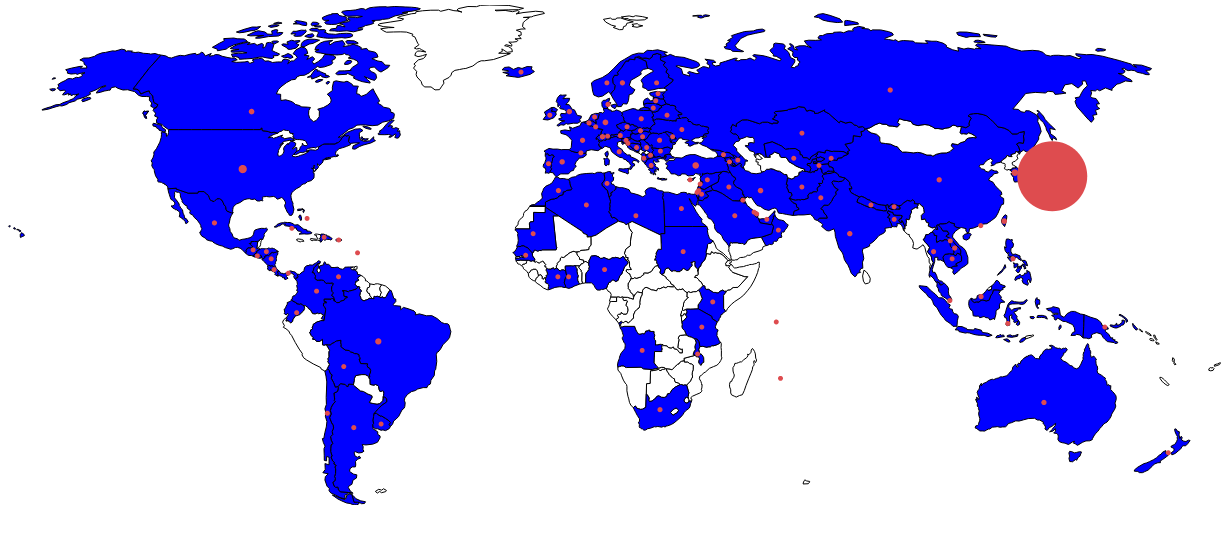
\includegraphics[width=1\columnwidth]{map.png}
% \caption{Countries}
% \label{fig:map}
% \end{figure}

\begin{figure}[!hbt]
\centering
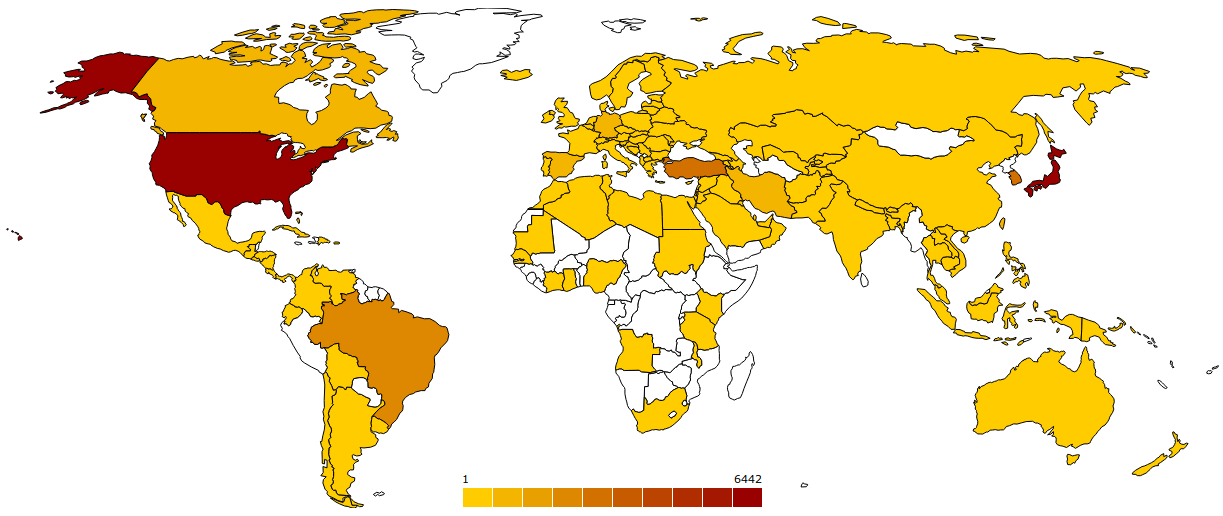
\includegraphics[width=1\columnwidth]{heatmap.png}
\caption{Map of vulnerable countries.}
\label{fig:heatmap}
\end{figure}



\subsection{Per-CERT statistics}

For each one of the affected countries, we mapped the vulnerable resources to the IPv4 space that is under the jurisdiction of the national CERTs\footnote{Note that in certain countries there are multiple CERTs}. Figure~\ref{fig:certs} shows the number of vulnerable resources --both DNS servers and domain names-- that each CERT is responsible for. 
Following the country-level pattern, the Japanese CERT is the one that hogs most of the vulnerable domains with more than 2-order of magnitude difference. Aside from JP-CERT, the distribution of vulnerable resources across CERT seems to follow a log-normal distribution. Thus, while there are some CERT than only have one vulnerable domain/IPv4 address, more than 50\% of the CERT are responsible for hundreds of vulnerable resources. 
\begin{figure}[!ht]
\centering
\begin{subfigure}[b]{0.45\columnwidth}
    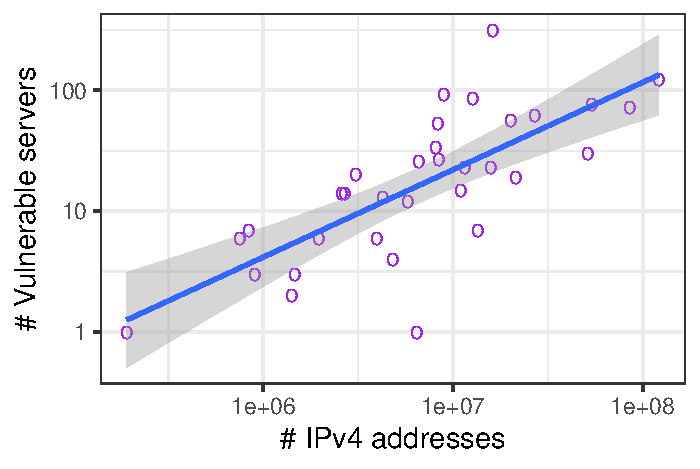
\includegraphics[width=\textwidth]{figs/certs_sizevsservers.pdf}
    \caption{Vulnerable DNS servers}
    \label{fig:size_servers_cert}
    \end{subfigure}
\hfill
\begin{subfigure}[b]{.45\columnwidth}
    \centering
    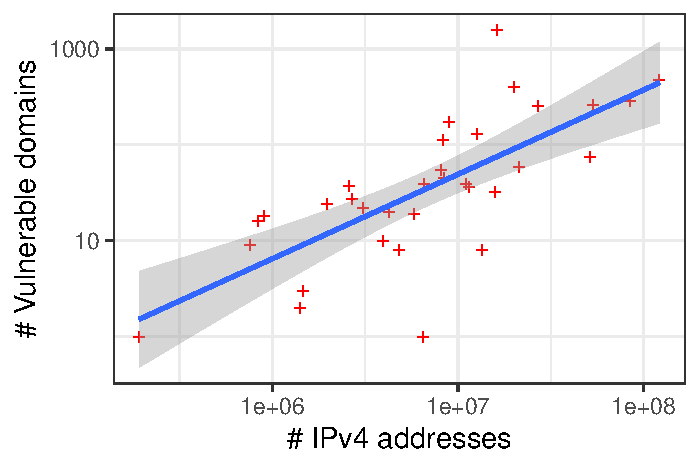
\includegraphics[width=\textwidth]{figs/certs_sizevsdomains.pdf}
    \caption{Vulnerable domains}
    \label{fig:size_domains_cert}
\end{subfigure}
\caption{Distribution of vulnerable resource per CERT size}
   \label{fig:size_cert}
\end{figure}



To further investigate these log-normal distribution, we estimated the size of each CERT by counting the amount of IPv4 addresses that are under their jurisdictions. Figure~\ref{fig:size_cert} plots the amount of vulnerable servers (Fig.~\ref{fig:size_servers_cert}) and the amount of vulnerable domains (Fig.~\ref{fig:size_domains_cert})) versus the size of the CERT for each one of the identified national CERTs.
As expected, larger CERTs accumulate higher number of vulnerable resources. However,we can also identify a few outliers. For instance, the CERT in Tunisia only had 1 vulnerable resource while having more than 6M IPv4 addresses under their responsibility. On the contrary, the CERT in Malasya with a similar number of IPv4 addresses, it had more than 200 vulnerable resources. 


\begin{figure*}[!hbt]
\centering
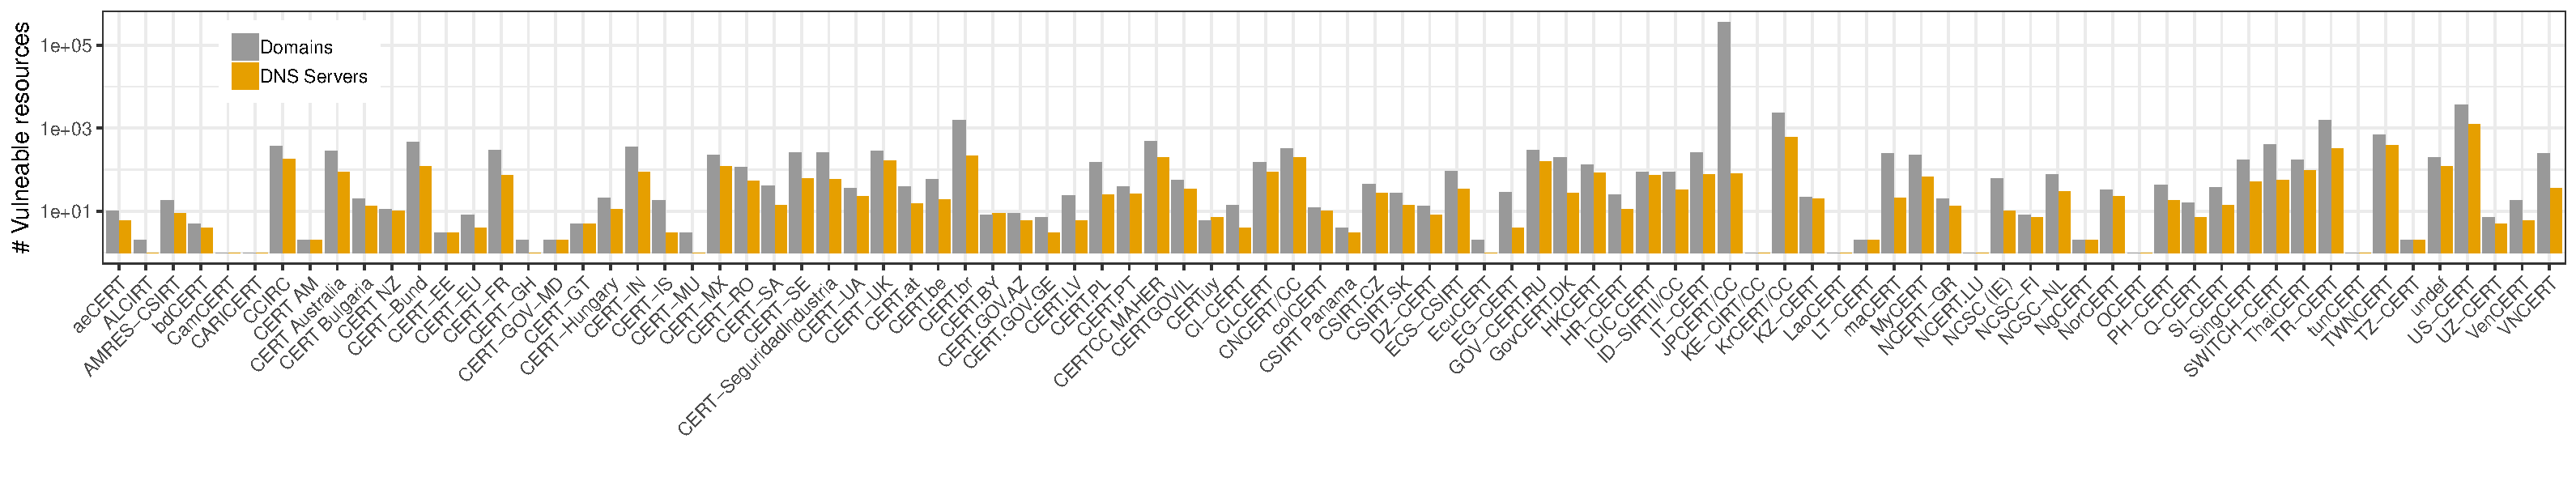
\includegraphics[width=1\textwidth]{certs.pdf}
\caption{Vulnerable resources per CERT}
\label{fig:certs}
\end{figure*}

\subsection{Per-AS statistics}
We continue by investigating distribution of vulnerable resources across different Autonomous Systems (AS). \autoref{fig:ip_pie} shows the number of vulnerable domains per authoritative server. 2 authoritative servers (119.82.8.252 and 119.82.8.251) are responsible for 80\% of vulnerable domains, while the 3rd server is responsible for 2.2\% of them. 

Those results are confirmed by per-AS analysis (\autoref{fig:ip_as_pie}). AS 33363 contains two main vulnerable authoritative servers and constitutes 83.9\% of vulnerable domains. 5 ASes containing the largest amount of vulnerable domains are responsible for 95.7\% of the total number of vulnerable resources. 

\begin{figure*}[!ht]
\begin{minipage}[t]{.33\textwidth}
    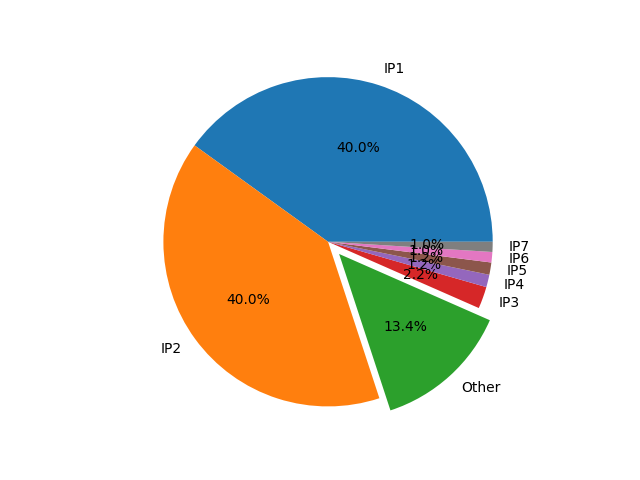
\includegraphics[width=1\columnwidth]{ip_pie_anonymous.png}
    \caption{Vulnerable IP addresses.}
    \label{fig:ip_pie}
\end{minipage}%
\begin{minipage}[t]{.33\textwidth}
    \centering
    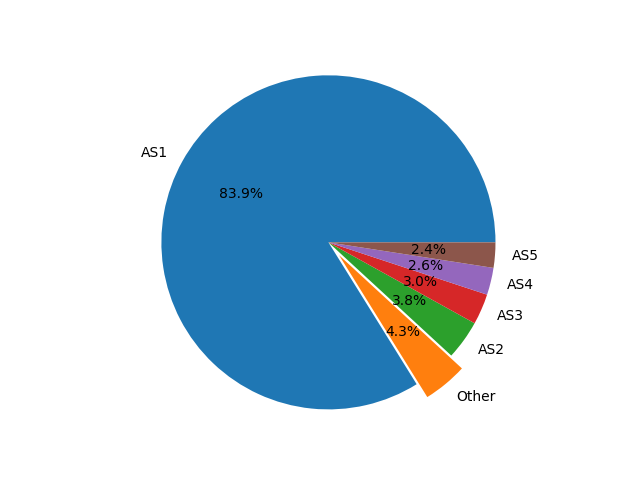
\includegraphics[width=1\columnwidth]{ip_as_pie_anonymous.png}
    \caption{Vulnerable Autonomous \\Systems.}
    \label{fig:ip_as_pie}
\end{minipage}%
\begin{minipage}[t]{.33\textwidth}
    \centering
    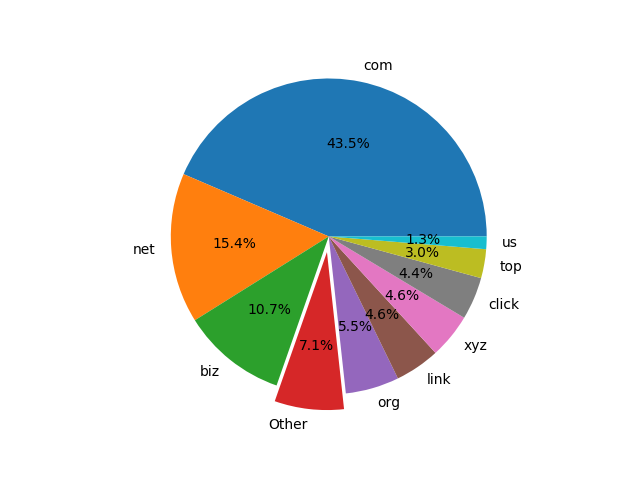
\includegraphics[width=1\columnwidth]{tld_pie.png}
    \caption{Vulnerable Top-Level Domains.}
    \label{fig:tld_pie}
\end{minipage}%

\end{figure*}



% \begin{figure}[!hbt]
% \centering
% 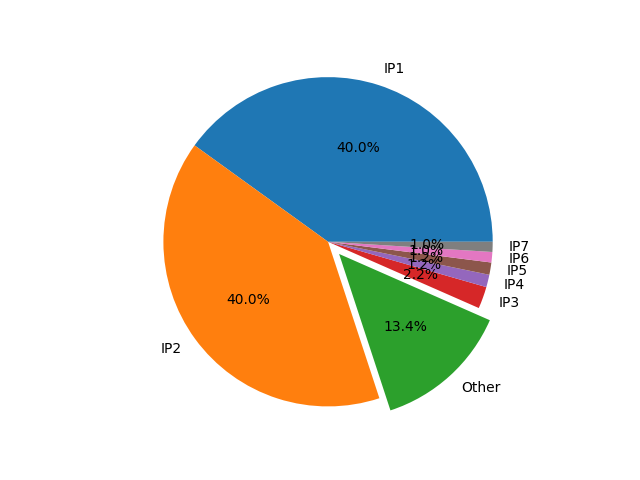
\includegraphics[width=.8\columnwidth]{ip_pie_anonymous.png}
% \caption{IP addresses}
% \label{fig:ip_pie}
% \end{figure}
% 
% \begin{figure}[!hbt]
% \centering
% 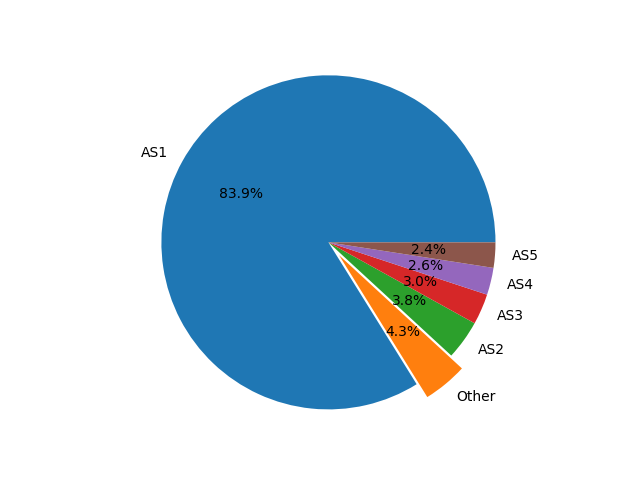
\includegraphics[width=.8\columnwidth]{ip_as_pie_anonymous.png}
% \caption{AS}
% \label{fig:ip_as_pie}
% \end{figure}



\subsection{Per-TLD statistics}

We analyse the Top Level Domains (TLD) of vulnerable domains (\autoref{fig:tld_pie}). The vast majority (69.6\%) belongs to the 3 most popular TLDs (.com, .net and .biz). We then compare the results against market share of each respective TLD (\autoref{fig:tld_market}). Interestingly, we observe the number of vulnerable .net and .biz domains significantly exceeding their overall market share. 

% \begin{figure}[!hbt]
% \centering
% 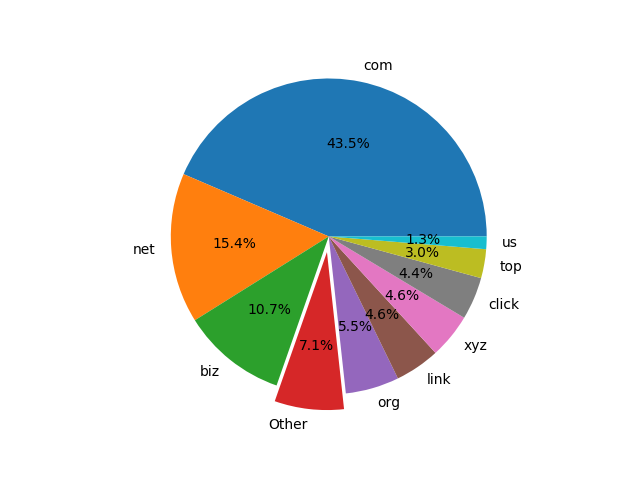
\includegraphics[width=.8\columnwidth]{tld_pie.png}
% \caption{TLD}
% \label{fig:tld_pie}
% \end{figure}

\begin{figure}[!hbt]
\centering
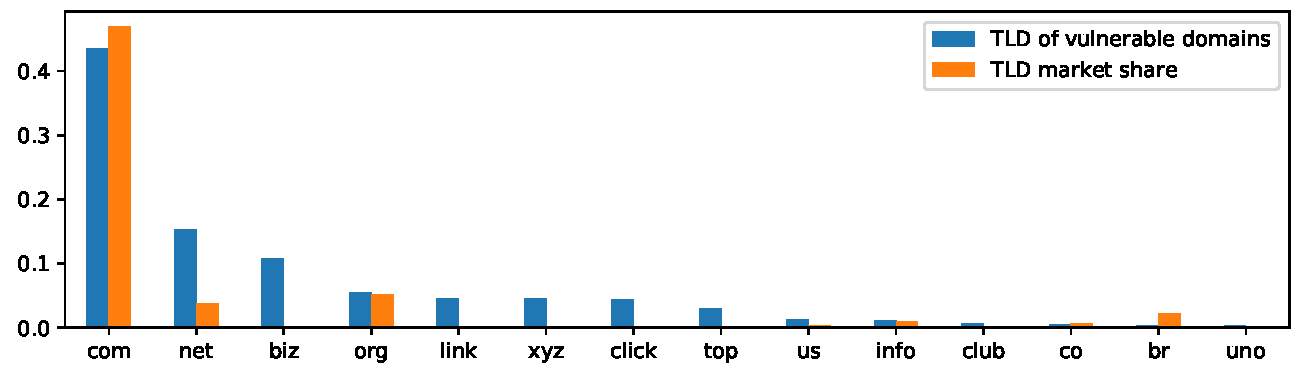
\includegraphics[width=1\columnwidth]{tld_market.pdf}
\caption{TLD market share}
\label{fig:tld_market}
\end{figure}



\michal{Should per-domain stats be here? Or in another subsection?}
\begin{figure}[!hbt]
\centering
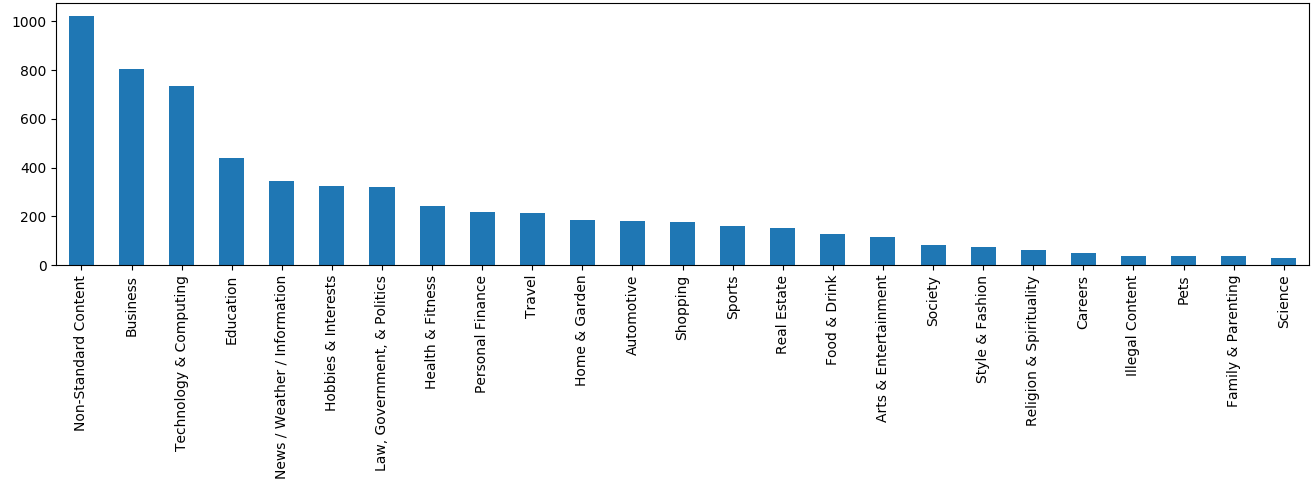
\includegraphics[width=1\columnwidth]{categories}
\caption{Domains Categorization}
\label{fig:categories}
\end{figure}

To determine the type of vulnerable domains, we perform classification using Webshrinker\footnote{\url{https://www.webshrinker.com/}}. Webshrinker uses machine learning to automatically classify domains using the IAB taxonomy\footnote{\url{https://support.aerserv.com/hc/en-us/articles/207148516-List-of-IAB-Categories}}. Out of 418,572 vulnerable domains, we were able to classify 6,175(1.5\%). \michal{How should we justify this? The rest were short-lived domains? Or domains without any content so we cannot classify?}
The results are shown on \autoref{fig:categories}. The most popular category consist of ``Non-Standard Content'' containing message boards, content servers and adult content. Surprisingly, the second most popular category is business containing several bank and government websites. We notice also a significant amount of domains belonging to educational and healthcare institutions. 
\michal{Shall we have a more in-depth analysis of the categories?}

\subsection{Popularity of affected domains}

Among the vulnerable domains we find 5089 domains present on Alexa 1M list in a period between April 2015 and November 2018. The most popular affected domains reached 266th place on the list. \autoref{fig:domains_cdf} presents cumulative distribution function of the positions reached  by the affected domains on the Alexa 1M list. 


\begin{figure}[!hbt]
\centering
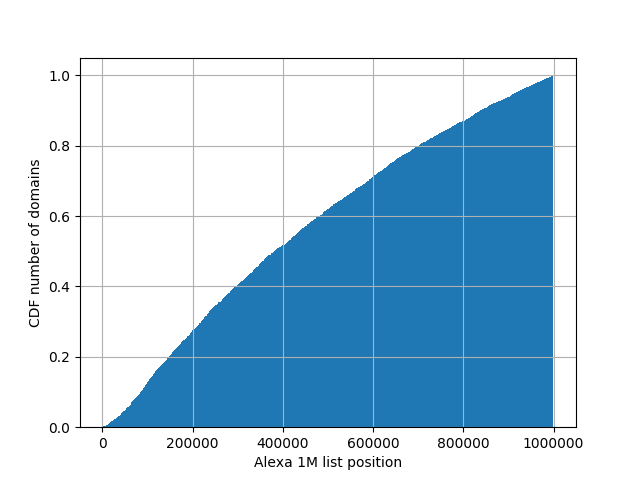
\includegraphics[width=.8\columnwidth]{domains_cdf.png}
\caption{Popularity of affected domains - CDF}
\label{fig:domains_cdf}
\end{figure}
